\documentclass{article}
\usepackage[en]{ukon-infie}
\usepackage[utf8]{inputenc}
\usepackage{algorithm2e}
\usepackage{amsmath}
\usepackage{graphicx}
\usepackage{hyperref}
% kann de oder en sein
% kann bubble break, topexercise sein

\Names{Jonas Probst, Simon Giebenhain}
\Lecture[AnaVis]{Analyse und Visualisierung von Informationen}
\Term{WS 2017/18}

\begin{document}
    \begin{ukon-infie}[24.01.18]{10}

        \begin{exercise}[p=6]{Gestalt Laws}  
        \question{}
        {
      	\begin{enumerate}
      	\item \textbf{Proximity}: In the left diagramm the points are percieved as clusters.
      	\item Similarity
      	\item \textbf{Connectedness}: In the right diagramm the points are not  percieved as clusters anymore, but as time-series data.
      	\item Continuity
      	\item \textbf{Figure and Ground}: The axes and points are clearly identified to be in the foreground.
      	\item Symmetry
      	\end{enumerate}
      	}
      	
      	\question{}
      	{
      		On the left hand side, the proximity of the points has the biggest influence on our perception. Therefore, it is easy to percieve them in clusters and ignore the time axis, instead of regarding them as time-series data.\\
      		On the right hand side the line connecting the data points underlines their chronological relation, which helps to see the diagramm as intended.
      	}
		\end{exercise}
		
		
		\begin{exercise}[p=2]{Pre-attentive Perception}
		\question{}
		{
		Pre-attentive perception describes a kind of perception, in which the user percieves the object of interest immediately, without spending any concious thoughts about it.
		}
		\newpage
		\question{}
		{
			One example would be locating your current postion on a map, e.g. in a navigation system, as it can be seen on the screenshot below. In such a case it is extremely helpful to have a clearly visibile marker enabeling preattentive perception, because often the map is loaded with details, making it hard to make out your location, without this obvious marker. Furthermore the view of the user continously jumps from his/her current location to his/her destination, when planning a route.\\
			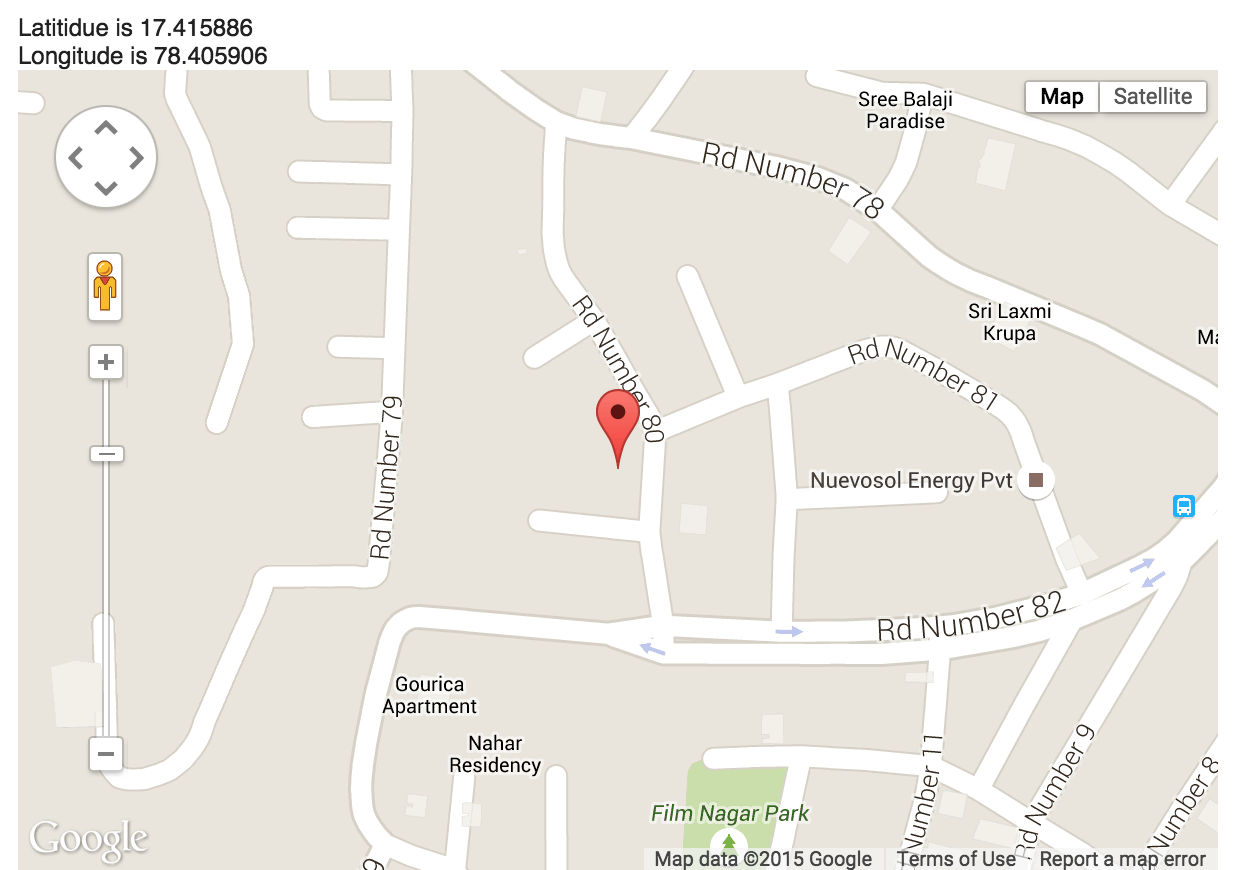
\includegraphics[scale=0.4]{preattentive_perception.png}
		}
		\end{exercise}
		
		\begin{exercise}[p=4]{Pixel-oriented Visualization}
		\question{}
		{
			Parallel coordinates visualization has problems with data like in Figure 1, because the graphs for different stocks will start to overlap, which will reduce legibility, so scalability is better for pixel-oriented visualization. But for smaller datasets with less graphs more detail can be shown in parallel coordinates.
		}
		\question{}
		{
			Recursive patterns help grouping data together that belongs together. \\
			For example if you have time data for one variable and you would show it line by line, at the start of a new line the first value would be far away from its preceding value at the end of the last line. So here a recursive pattern would be useful.
		}
		\end{exercise}

		\begin{exercise}[p=5]{Expressiveness and Effectiveness}
			\question{}
			{
				\textbf{Expressiveness:} The visualization is expressive when it shows all the information it's supposed to, but no additional information which might be misleading or wrong.\\\\
				\textbf{Effectiveness:} A visualization is effective when it's easy and quick to interpret and not too complicated to render.
			}
			\newpage
			\question{}
			{
				\textbf{Counter example for Expressiveness:}\\
				The temperature values are missing for a lot of regions.\\
				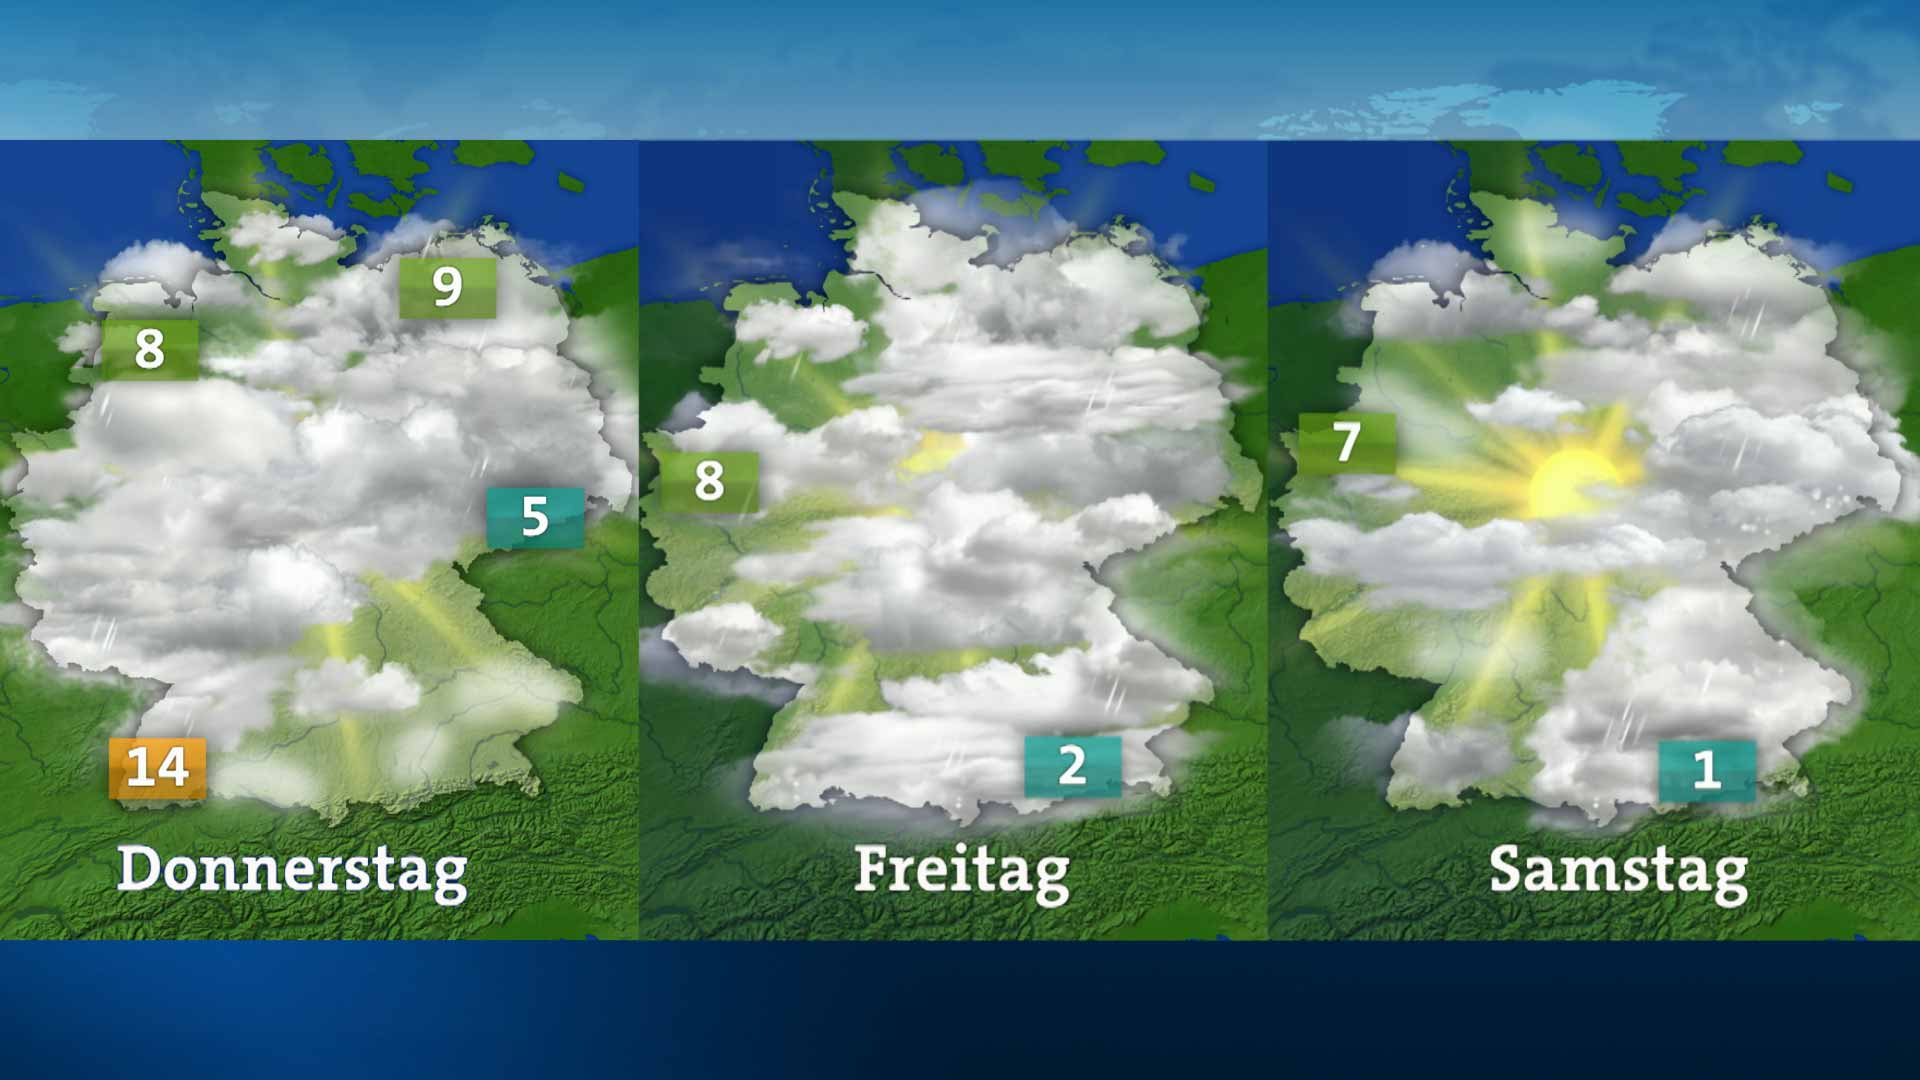
\includegraphics[scale=0.2]{effectiveness.jpg}\\
				
				\textbf{Counter example for Effectiveness:}\\
				All values are given, but it's difficult to get any significant information out of the chart.\\
				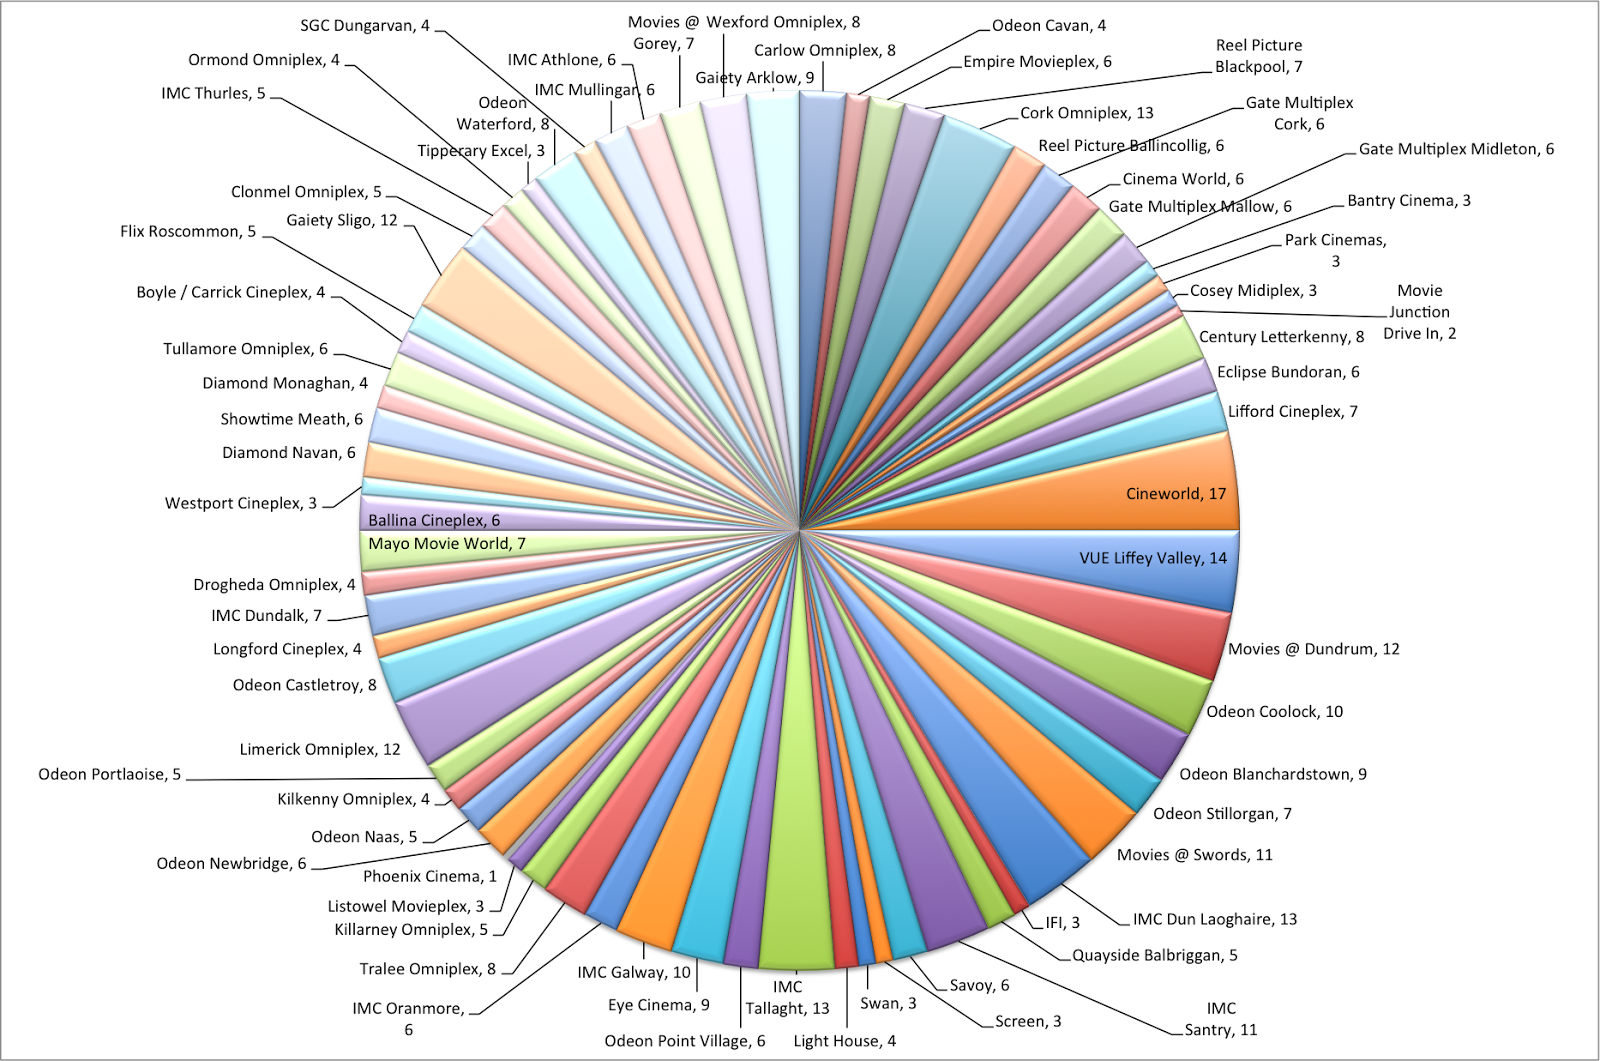
\includegraphics[scale=0.2]{expressiveness.png}
			}
			
		\end{exercise}		
		
		\begin{exercise}[p=5]{Visual Variables}
			\question{}
			{
				Position\\
				Mark/Shape\\
				Size (Length, Area and Volume)\\
				Brightness\\
				Color\\
				Orientation\\
				Texture\\
				Motion\\
			}
			
			\question{}
			{
				Selective: A set of marks with the same value of a variable is perceived as a group.\\
				Associative: Objects can be perceived a being in a group despite differences in this variable.\\
				Quantitative: The difference between two values of a variable can be interpreted numerically.\\
				Order: Objects can be ordered according to this variable.\\
				Length: The amount of different values of a variable that can be perceived.
			}
			
			\question{}
			{
				That depends a lot on whether quantitative, ordinal or nominal data should be visualized. Position is always a good starting point. It's useful to keep this chart in mind:\\
				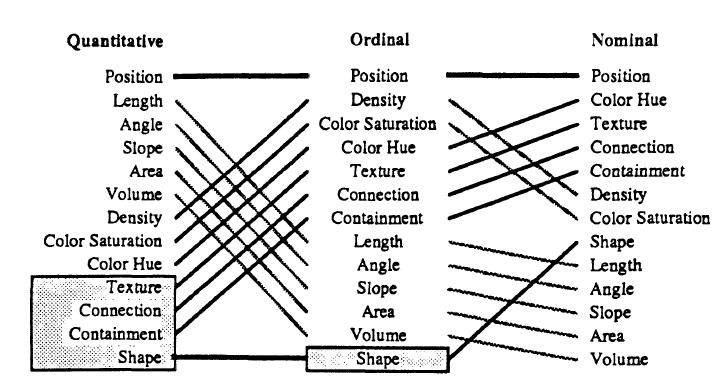
\includegraphics[scale=0.6]{order.jpg}
			}
		\end{exercise}
		
\end{ukon-infie}
\end{document}
